\documentclass[tikz]{standalone}
\usetikzlibrary{patterns}
\usetikzlibrary{arrows}
\usetikzlibrary{decorations.shapes,decorations.markings,decorations.pathreplacing}

\tikzset{
    set arrow inside/.code={\pgfqkeys{/tikz/arrow inside}{#1}},
    set arrow inside={end/.initial=>, opt/.initial=},
    /pgf/decoration/Mark/.style={
        mark/.expanded=at position #1 with
        {
            \noexpand\arrow[\pgfkeysvalueof{/tikz/arrow inside/opt}]{\pgfkeysvalueof{/tikz/arrow inside/end}}
        }
    },
    arrow inside/.style 2 args={
        set arrow inside={#1},
        postaction={
            decorate,decoration={
                markings,Mark/.list={#2}
            }
        }
    },
}
\begin{document}
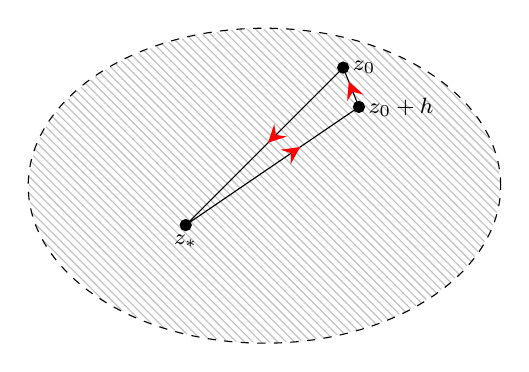
\begin{tikzpicture}
\draw[pattern=north west lines,pattern color=gray!50,draw=white] (0,0) ellipse(3 and 2);
\draw[dashed] (0,0) ellipse (3 and 2);
\draw[fill] (-1,-0.5) circle (2pt) node[below,font=\footnotesize] {$z_{\ast}$} -- (1.2,1) circle (2pt) node[right,font=\footnotesize]{$z_0+h$} -- node[midway,font=\footnotesize] (n1) {} (1,1.5) circle (2pt) node[right,font=\footnotesize]{$z_0$}  -- (-1,-0.5) [arrow inside={end=stealth,opt={red,scale=2}}{0.3,0.53,0.8}];
%\draw[->] (1,-0.5) node[below]{$[z_{\ast},z]$} -- (n1);

\end{tikzpicture}
\end{document}